\documentclass[12pt]{article}
\usepackage{times} 			% use Times New Roman font

\usepackage[margin=1in]{geometry}   % sets 1 inch margins on all sides
\usepackage[hidelinks]{hyperref}               % for URL formatting
\usepackage[pdftex]{graphicx}       % So includegraphics will work
\setlength{\parskip}{1em}           % skip 1em between paragraphs
\usepackage{indentfirst}            % indent the first line of each paragraph
\usepackage{datetime}
\usepackage[small, bf]{caption}
\usepackage{listings}               % for code listings
\usepackage{xcolor}                 % for styling code
\usepackage{multirow}

%New colors defined below
\definecolor{backcolour}{RGB}{246, 246, 246}   % 0xF6, 0xF6, 0xF6
\definecolor{codegreen}{RGB}{16, 124, 2}       % 0x10, 0x7C, 0x02
\definecolor{codepurple}{RGB}{170, 0, 217}     % 0xAA, 0x00, 0xD9
\definecolor{codered}{RGB}{154, 0, 18}         % 0x9A, 0x00, 0x12

%Code listing style named "gcolabstyle" - matches Google Colab
\lstdefinestyle{gcolabstyle}{
  basicstyle=\ttfamily\small,
  backgroundcolor=\color{backcolour},   
  commentstyle=\itshape\color{codegreen},
  keywordstyle=\color{codepurple},
  stringstyle=\color{codered},
  numberstyle=\ttfamily\footnotesize\color{darkgray}, 
  breakatwhitespace=false,         
  breaklines=true,                 
  captionpos=b,                    
  keepspaces=true,                 
  numbers=left,                    
  numbersep=5pt,                  
  showspaces=false,                
  showstringspaces=false,
  showtabs=false,                  
  tabsize=2
}

\lstset{style=gcolabstyle}      %set gcolabstyle code listing

% to make long URIs break nicely
\makeatletter
\g@addto@macro{\UrlBreaks}{\UrlOrds}
\makeatother

% for fancy page headings
\usepackage{fancyhdr}
\setlength{\headheight}{13.6pt} % to remove fancyhdr warning
\pagestyle{fancy}
\fancyhf{}
\rhead{\small \thepage}
\lhead{\small HW\#0, Huang}  % EDIT THIS, REPLACE # with HW number
\chead{\small DATA 440, Fall 2022} 

%-------------------------------------------------------------------------
\begin{document}

% EDIT THE ITEMS HERE
\begin{centering}
{\large\textbf{HW\#0 - Homework Report}}\\ 
Sofia Huang\\
09/02/2022 (due 09/13/2022)\\
\end{centering}

%-------------------------------------------------------------------------

% The * after \section just says to not number the sections
\section*{Part 1, Question 1}

\emph{You may copy the question into your report, but make sure that you make it clear where the question ends and your answer begins.}

\subsection*{Answer}

\emph{All figures must have a caption and must be referenced in the text. Example below.}

Figure \ref{fig:sine-graph} shows the graph of the trigonometry function \(y = sin x\).

\begin{figure}[h]
    \centering
    % trim and clip are used to crop the image, trim=left bottom right top
    % width sets max width, height will be scaled appropriately
    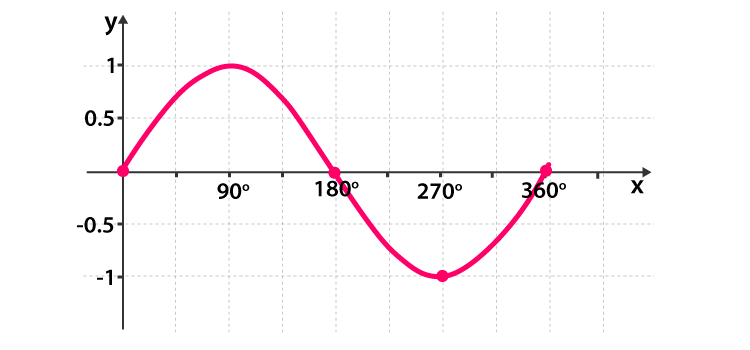
\includegraphics[trim=0 20 10 50, clip, width=\textwidth] {Sine-Graph.png}
    \caption{Sine Graph}
    \label{fig:sine-graph}
\end{figure}

\emph{If you want to include code in your report, you can insert a screenshot (if it's legible), or you can copy/paste the code into a listings environment. There are examples below and more information is available at \url{https://www.overleaf.com/learn/latex/code_listing}.}

Listing \ref{lst:copy} is an example of directly copying code into the LaTeX document and having the listings package perform syntax highlighting. Listing \ref{lst:import} is an example of importing the code from a file rather than copying it in.

%Python code highlighting
\begin{lstlisting}[language=Python, caption=Python example copied into the LaTeX, label=lst:copy]
a = 1

try:
    b = int(input("Please enter a number to divide a"))
    a = a/b
    print("Success a=",a)
except ZeroDivisionError:
    print("The number you provided cant divide 1 because it is 0")
except ValueError:
    print("You did not provide a number")
except:
    print("Something went wrong")
\end{lstlisting}

%Importing code from file
\lstinputlisting[language=Python, caption=Python sample code loaded from file, label=lst:import]{divide-number.py}

Table \ref{tbl:simple} shows a simple example table.  Table \ref{tbl:confusion} shows an example confusion matrix (you'll see this term later) from \url{https://en.wikipedia.org/wiki/Confusion_matrix}. This employs rows that span multiple columns (multicol) and columns that span multiple rows (multirow). 

\begin{table}[h]
\centering
\caption{Simple Table}
\label{tbl:simple}
\begin{tabular}{|l|l|l|}
\hline
\textbf{Week} & \textbf{Date} & \textbf{Topic} \\ \hline \hline
1 & Sep 1, 6 & Introduction to Web Science and Web Architecture \\ \hline
2 & Sep 8, 13 & Introduction to Python \\ \hline
3 & Sep 15, 20 & Introduction to Info Vis with R, Python \\ \hline
4 & Sep 22, 27 & Measuring the Web \\ \hline
\end{tabular}
\end{table}

\begin{table}[h]
\centering
\caption{Example Confusion Matrix from Wikipedia}
\label{tbl:confusion}
\begin{tabular}{l|l|c|c|}
\multicolumn{2}{c}{}&\multicolumn{2}{c}{Actual}\\
\cline{3-4}
\multicolumn{2}{c|}{}&Cat&Dog\\
\cline{2-4}
\multirow{2}{*}{Predicted}& Cat & 5 (TP) & 3 (FP)\\
\cline{2-4}
& Dog & 2 (FN) & 3 (TN) \\
\cline{2-4}
\end{tabular}
\end{table}

\subsection*{Discussion}

For the first part of the homework assignment I followed the instructions given to replace various figures and code blocks to get familiar with Latex. 

\section*{Part 2, Question 1}

\subsection*{Answer}

\begin{lstlisting}[language=bash, caption=Permissions on directory, label=lst:copy]
(base) sofiahuang@Sofias-MacBook-Pro Desktop % chmod 700 data440 
(base) sofiahuang@Sofias-MacBook-Pro Desktop % ls -l data440
total 8
-rwx------@ 1 sofiahuang  staff  45 Sep  6 10:26 test.txt
\end{lstlisting}

\subsection*{Discussion}

I googled how to change the permissions on a directory using the Terminal and I came across \lstinline{chmod}. The $700$ after the command denotes what the permissions are being changed to. The first digit placeholder represents the user permissions, the second is for groups, and the third is for others. Then, the actual number represents the sum of the type of permissions: 4 - read, 2 - write, 1 - execute, 0 - none. So, to give the user permission to read, write, and execute, we add $4 + 2 + 1 = 7$. Then, everyone else (groups and others) is assigned 0 for no permissions.

\section*{Part 2, Question 2}

\subsection*{Answer}

\begin{lstlisting}[language=bash, caption=Unix commands, label=lst:copy]
(base) sofiahuang@Sofias-MacBook-Pro data440 % wc -l test.txt
       5 test.txt

(base) sofiahuang@Sofias-MacBook-Pro data440 % echo "CS 800" >> test.txt; cat test.txt
CS 800
CS 432
CS 725
MATH 212
MATH 32
CS 800

(base) sofiahuang@Sofias-MacBook-Pro data440 % grep CS test.txt
CS 800
CS 432
CS 725
CS 800

(base) sofiahuang@Sofias-MacBook-Pro data440 % grep -c CS test.txt
4

(base) sofiahuang@Sofias-MacBook-Pro data440 % sort test.txt
CS 432
CS 725
CS 800
CS 800
MATH 212
MATH 32

(base) sofiahuang@Sofias-MacBook-Pro data440 % sort -k2 test.txt
MATH 212
MATH 32
CS 432
CS 725
CS 800
CS 800

(base) sofiahuang@Sofias-MacBook-Pro data440 % sort -k2 -n test.txt

MATH 32
MATH 212
CS 432
CS 725
CS 800
CS 800

(base) sofiahuang@Sofias-MacBook-Pro data440 % sort test.txt | uniq -c

   1 CS 432
   1 CS 725
   2 CS 800
   1 MATH 212
   1 MATH 32
\end{lstlisting}

\subsection*{Discussion}

For each command, I used the \lstinline{man} command in the Terminal to find out its purpose.

The \lstinline{wc -l} command returns the line count (specified by the \lstinline{-1} parameter) of the input file, which was 5. 

The \lstinline{echo} command writes arguments to the standard output, which is what you see returned in the Terminal after executing commands that have an output. The \lstinline{>>} symbol is used for output redirection, which is how the output, "CS 800", from the \lstinline{echo} command is able to be appended to the input file. Then, the semicolon is used to run multiple Linux commands in one line (using a semicolon, all commands are run, regardless if the previous executed successfully or not). The \lstinline{cat} command is used to read and print the specified file to the standard output so we can check and see that "CS 800" was indeed appended to the text file.

The \lstinline{grep} command searches the file and returns the lines that match the given patterns/regular expressions. In this example, we looked for "CS" and all of the lines in the test file with that expression were returned.

When you add the \lstinline{-c} parameter to the \lstinline{grep} command, the output returns the count of matches from the input file, which in this case was 4.

The \lstinline{sort} command sorts the input file by line, lexicographically.

When the \lstinline{-k2} parameter is added, the input file is sorted by the second column. However, still in lexicographical order, which is why "212" is before "32".

The \lstinline{-n} parameter tells the command to sort numerically. Combined with the \lstinline{-k2} parameter, we see that the file is sorted by the second column in ascending numerical order.

Lastly, the pipe command combine multiple commands so that the output of one is the input of the next. The \lstinline{uniq} command compares each adjacent line and filters out duplicates. It is best to sort the input file first since this command compares adjacent lines, so for example, if the first and last line (not adjacent) are duplicates of each other, this will not be detected and both lines will be outputted. By adding the \lstinline{-c} parameter, the count of each line is added to the output. Since "CS 800" appears twice in the file, there is a "2" in front of it.

\clearpage

\section*{Part 3, Question 1}

\subsection*{Answer}

\begin{lstlisting}[language=bash, caption=Running get\_tweets.py, label=lst:copy]
(base) sofiahuang@Sofias-MacBook-Pro data440 % python3 get_tweets.py "national park"
25 tweets written to tweets.jsonl for query "national park lang:en has:links -is:retweet"
\end{lstlisting}

\begin{lstlisting}[language=bash, caption=tweets.jsonl output snippet, label=lst:copy]
(base) sofiahuang@Sofias-MacBook-Pro data440 % jq . tweets.jsonl 
{
  "text": "Come tour with us!\nThe Mole National Park is a place to visit and experience wildlife in the Savanna Region of Ghana.\nNature is beautiful, Yaa Asantewaa Tours is here for you!!\nContact us anytime for adventurous and exciting tours.\n0209079288\nyaaahendea@gmail.com\n#pulseofafrica https://t.co/YhUHPGdUTO",
  "id": "1567876436031062018",
  "entities": {
    "annotations": [
      {
        "start": 18,
        "end": 40,
        "probability": 0.2616,
        "type": "Place",
        "normalized_text": "The Mole National Park"
      },
      {
        "start": 93,
        "end": 115,
        "probability": 0.8115,
        "type": "Place",
        "normalized_text": "Savanna Region of Ghana"
      },
      {
        "start": 139,
        "end": 157,
        "probability": 0.5972,
        "type": "Place",
        "normalized_text": "Yaa Asantewaa Tours"
      }
    ],
 ...
\end{lstlisting}


\subsection*{Discussion}

After I created a Developer Account and installed twarc, I had to find where the config file was loacted on my computer that contained my keys in order to run \lstinline{get_tweets.py}. Once I found it and changed the file path in the python script, I was able to run and get tweets (I chose to use the keywords "national park"). In order to display the JSONL file in an organized manner, I installed and used the \lstinline{jq} package, which is a command-line JSON file processor.

\section*{Part 3, Question 2}

\subsection*{Answer}

\begin{lstlisting}[language=bash, caption=tweets\_info.txt output snippet, label=lst:copy]
(base) sofiahuang@Sofias-MacBook-Pro data440 % python3 process_tweets.py < tweets.jsonl > tweets_info.txt
(base) sofiahuang@Sofias-MacBook-Pro data440 % cat tweets_info.txt
1567876436031062018	2022-09-08T14:04:06.000Z	yaaasantewaa_ad	0
  Brand Category: Sports & Fitness Business
  Brand Category: Travel & Transportation Business
  Entities [Entity Service]: Travel
  Interests and Hobbies Category: Destinations
  Interests and Hobbies Category: Outdoors
  Interests and Hobbies: National parks
  Unified Twitter Taxonomy: National parks
  https://twitter.com/yaaasantewaa_ad/status/1567876436031062018/photo/1
\end{lstlisting}

\subsection*{Discussion}

For this question I ran the line of code provided in the instructions and then used the \lstinline{cat} command to show the .txt file that was created. Above is a snippet of the output showing the tweet information.

\section*{References}

\emph{Every report must list the references that you consulted while completing the assignment. If you consulted a webpage, you must include the URL.}

\begin{itemize}
    \item {StackExchange - Can't edit a downloaded template from Overleaf on TexMaker} \url{https://tex.stackexchange.com/questions/593363/cant-edit-a-downloaded-template-from-overleaf-on-texmaker}
    \item {How to Create a Folder in Github Repos in 4 Simple Steps}
    \url{https://www.alpharithms.com/how-to-create-a-folder-in-github-repos-463022/}
    \item {Linux Commands} \url{https://linuxconfig.org/linux-commands-cheat-sheet}
    \item {Latex Inline Code} \url{https://tex.stackexchange.com/questions/286094/insert-code-keywords-inline}
    \item{Linux chmod} \url{https://www.computerhope.com/unix/uchmod.htm}
\end{itemize}

\end{document}


